\renewcommand{\arcsec}{$^{\prime\prime}$} %redundant command definition, but needed for thesis template
\renewcommand{\arcmin}{$^{\prime}$}
\newcommand{\rts}[1]{{\color{violet} RTS: #1}} % RTS comment
\newcommand{\jdp}[1]{{\color{red} JDP: #1}} % JDP comment
\newcommand{\cck}[1]{{\color{brown} CCK: #1}} % CCK comment
\newcommand{\amy}[1]{{\color{cyan} ARW: #1}}

% #1- element #2- ionization state #3 -wavelength in angstroms
\newcommand{\spectralline}[3]{#1\,{\sc #2}\,#3\,\AA \,}
\newcommand{\ov}{\spectralline{O}{v}{627.8}}
\newcommand{\mgxbright}{\spectralline{Mg}{x}{609.8}}
\newcommand{\hei}{\spectralline{He}{i}{584.3}}
\newcommand{\heii}{\spectralline{He}{ii}{304}}



\title{First Flight of the EUV Snapshot Imaging Spectrograph (ESIS)}

\author{Jacob D. Parker}
%\author{Roy Smart}
%\author{Charles Kankelborg}
%\author{Amy Winebarger}
%\author{Nelson Goldsworth}

\begin{abstract}
  	The Extreme-ultraviolet Snapshot Imaging Spectrograph (ESIS) was launched on a sounding rocket from White Sands Missile Range on September 30, 2019.
  	ESIS is a Computed Tomography Imaging Spectrograph (CTIS) designed to capture both spectral and spatial information simultaneously over a large field of view to provide velocity information on small scale transient events that are prevalent at transition region temperatures.
  	In this paper, we review the ESIS instrument, mission, and the data captured.
  	We demonstrate how this unique data set can be interpreted qualitatively, and further present some initial quantitative inversions of the data.
  	Using a Multiplicative Algebraic Reconstruction technique we are able to combine information from all four ESIS channels into a single spatial-spectral cube at every exposure.
  	We analyze two small explosive events in the \ov spectral line with jets  near $\pm$100 km/s that evolve on 10 s time scales and vary significantly over small spatial scales.
  	In the 5 minutes of observing time, ESIS captured tens of the small events across the $\approx$11' field of view, as well as several larger extended eruptions, demonstrating the advantage of CTIS instruments over traditional slit spectrographs in capturing the spatial and spectral information of dynamic solar features across large fields of view.
  	
\end{abstract} 

\section{Introduction}

    The solar transition region (TR) is the solar plasma that exists at temperatures between the
    dense, cool (20,000 K) solar chromosphere and the tenuous, million-degree corona. 
    Initially, the transition region was viewed as simply the thin interface region between the chromosphere and corona, where the temperature of the plasma dramatically increased two orders of magnitude over tens of kilometers. 
    Though undoubtedly this type of transition region exists in hot coronal loops, the concept of the transition region has been expanded over the last twenty years to include a dynamic and complicated three-dimensional geometry. 
    It is in the low transition region where the magnetic pressure begins dominate the plasma pressure. The transition region is rife with magnetically driven phenomena such as explosive events \cite[e.g.,][]{dere1991} and microflares \citep{gontikakis2012} and associated flows of 100+ km/s.  \amy{this is from proposal, I will add more description and references and basically re-write.}
    
    Investigations of TR events to date are severely limited by available observational capabilities. 
    Historically, slit spectrographs have been used to study the solar atmosphere.   
    Two-dimensional spectral information must be built by rastering the slit over the region of interest, which takes much longer than the timescales of TR phenomena and confuses whether events are temporally evolving or varying spatially.  
    One solution to simultaneously capture spatial and spectral information over a large field of view is to use an slitless imaging spectrograph.  
    The data from these instruments, sometimes called overlapograms, have spatial and spectral information overlapped in the dispersive direction, requiring the data to be inverted or unfolded.  
    
    The difficulty in unfolding the data has limited its usefulness for extended astrophysical objects like the Sun. 
    Only two satellite missions have routinely captured solar slitless spectrograph data; {\it Skylab} \citep{Tousey1973} and the Res-K instrument of the Russian KRONOS-I mission \citep{Zhitnik1998}, though others have been recently developed and proposed \citep{winebarger2019,golub2020}. Additionally, the currently-operating Extreme-ultraviolet Imaging Spectrograph (EIS; \citet{culhane2007}) on the {\it Hinode} mission \citep{kosugi2007} includes 40\arcsec and 266\arcsec slots that can produce overlappogram data.  Though this data is not often taken for scientific analysis, it has been used as a flare trigger and since analyzed to aid in interpretation of impulsive phase of solar flares \citep{harra2017,harra2020}.
    In addition to these satellite observatories, there have been several solar observations with slitless spectrographs on sounding rocket flights, including the Multi-Order Solar EUV Spectrograph (MOSES) instrument by Kankelborg and collaborators \citep{Kankelborg01,Fox10}.
     MOSES captured the zero and plus and minus one order of the \heii line simultaneously. Doppler shifts were then detected as the spectral displacements in opposite directions in the $\pm$ 1 orders.
    
    Slitless spectrograph data can be thought of as a projection of a spatial-spectral data cube, $I(x,y,\lambda)$, onto a two dimensional detector.  
    To invert temperature or density information from slitless spectrograph data, only a single projection of this cube is required, as demonstrated by \cite{winebarger2019}.  
    However, to disentangle quantitative velocity information from slitless spectrograph data, additional projections of the data cube with different relative dispersive directions is necessary.  
    An instrument that captures multiple projections of the spatial-spectral data cube is called a Computed Tomography Imaging Spectrograph (CTIS).  MOSES is an example of a CTIS, as it captured two projections in the $\pm$ 1 orders.  
    
    In 2013, the Extreme-ultraviolet Snapshot Imaging Spectrograph (ESIS) was proposed to the NASA Low Cost Access to Space (LCAS) program and subsequently selected.  
    ESIS is a CTIS with four unique projections of the spatial-spectral data cube and is designed to capture velocity information in small-scale reconnection events in the \ov emission line that is formed in the solar transition region.  
%    ESIS was designed to be flown on the opposite side of the MOSES optics bench with the intention of both instruments gathering data simultaneously.   
    The ESIS mission was launched from White Sands Missile Range on September 30,  2019; this paper is a description of the ESIS mission, data and preliminary results.  
 %   Unfortunately MOSES was  not operational during the flight  and will not be discussed further.  
    The ESIS experiment, target, and flight is described in Section 2.  
    Section 3 provides information on the data processing.  Preliminary results are given in Section 4; these include both qualitative and quantitative measures of small-scale velocity events in the solar transition region.  The ESIS mission was successful in  observing tens of small-scale reconnection events over the short rocket flight, as well as demonstrating the usefulness of CTIS observations and developing the analysis techniques required to interpret this unique data.
%\jdp{I'm not sure why these comments about MOSES are relevant.  This is written like it is a review of mission success.}
%\amy{you mean the comments just in this paragraph about it not being operational?  We could remove the two sentences that discuss MOSES from this paragraph, but I was thinking because it was originally proposed to fly with MOSES and constrained in design to fly with MOSES had some impact on its design?  But completely up to you. I have commented them out.} 


\section{ESIS Mission}

In this section we provide an overview of the ESIS experiment as well as the time and conditions of the ESIS rocket launch and subsequent data collection.   

	\subsection{The Experiment}
	  	
    	The full ESIS experiment includes an optical instrument, a set of detectors, an on board data acquisition system, and ground support equipment and is described in great detail in the preceding paper \citep{ESIS}.
    	The ESIS optical design consists of a single parabolic primary mirror, an octagonal field stop placed at an intermediate focal plane, and 4 spherical diffraction gratings each with their own corresponding CCD detector.
    	Incoming light is focused by the primary mirror onto the octagonal field stop. 
    	The octagonal field stop is $\approx$ 5 mm wide, which is equivalent to roughly 11\arcmin \  when projected onto the sky. 
    	The light that exits the field stop is reimaged  by the four spherical diffraction gratings onto their own CCD.
    % 	operated in frame-transfer mode. Details like this are in the instrument paper 
    	The portion of the solar spectrum that is captured by each detector ranges from \hei to \ov.
    	
        \begin{figure}[ht]
			\begin{center}
				% \includegraphics{}
				\caption{Figure showing each ESIS projection, in an array, with solar.  JDP working on it.}
				\label{fig:level_1_array}
			\end{center}
		\end{figure}

    	
    	
    	Each grating and detector pair, referred in this paper as a channel, is itself an imaging spectrograph.  
    	The channels are arrayed at $45^{\circ}$ increments about the axis of symmetry of the paraboloidal primary mirror such that each channel disperses the solar image a different direction. 
    	Hence, each of these channels capture a unique projection of the spatial spectral cube, shown in Figure \ref{fig:level_1_array}. 
    	As shown, each channel captures the Sun imaged through the octagon and dispersed at different relative angles with respect to solar north. Combining these four channels creates a CTIS. Exposures from all four channels are gathered nearly simultaneously by triggering the frame transfer in three of the cameras by a single ``master'' camera. 
    	The ESIS instrument currently has 4 channels, but is built to accommodate up to 6 (limited by interference with the optical bench).

    	
        The dark current in the ESIS cameras is reduced by cooling detectors to low temperatures. 
        The CCDs in the ESIS cameras are mounted in a copper carrier, which is connected via a copper strap to a cold block.  
        The cold block is cooled prior during testing and prior to flight to -120 $^{\circ}$C.  This cold block acts as a thermal reservoir to maintain the CCD temperature during the $\sim$ 10 minute rocket flight.   
        ESIS exposures are transferred via spacewire to an on-board data acquisition system. During ground testing, including alignment, cameras can be commanded individually or collectively and images displayed via ethernet connection to an Operational Ground Support Equipment (GSE) computer.  
        During flight, ESIS is designed to operate autonomously, though commands can be uplinked if required.  
        Exposures are buffered, downlinked, and displayed in near real time on the Operational GSE.   These images can be used to make pointing corrections during flight if needed. \amy{This may be too much information, but I wanted to beef up this section.  
        Also, wanted to highlight  that ESIS isn't just an optical system, it is optical + on board electronics + ground support equipment.}
	
    
	\subsection{Launch and Data Collection} 
		\begin{figure}[ht]
			\begin{center}
				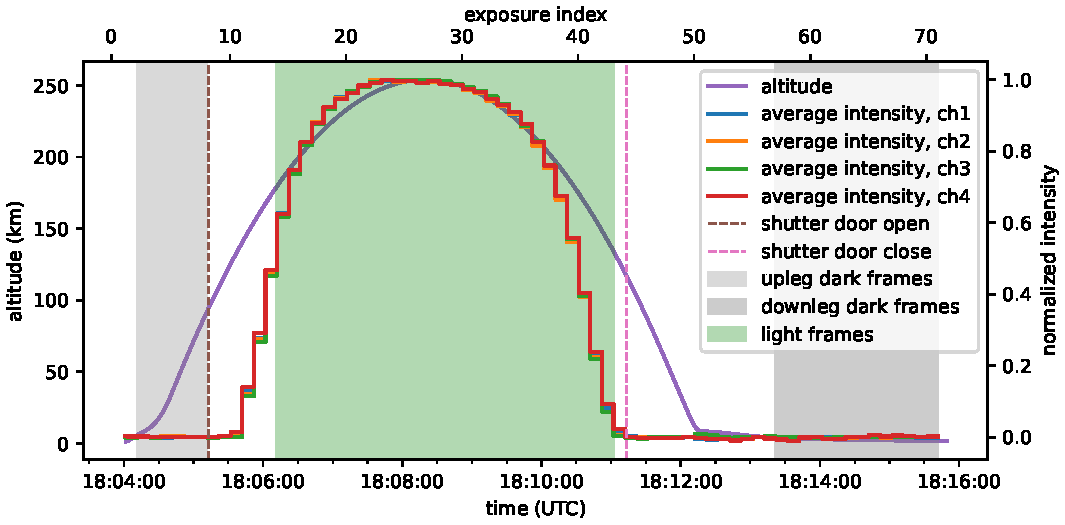
\includegraphics{figures/signal_and_altitude_vs_time}
				\caption{The altitude of the ESIS rocket determined from White Sands Missile Range radar data as a function of elapsed time from launch.  The event times listed in Table~\ref{tab:timeline} are labeled.}
				\label{fig:timeline}
			\end{center}
		\end{figure}

\amy{Roy: can you change the text in Figure 2 to be "lights" instead of "signal"}. \rts{Changed it to `light frames' and also changed it to `upleg/downleg dark frames' to match.}

		ESIS was launched at 18:04:00~UTC \rts{\timeMissionStart~UTC} on September 30, 2019 \rts{\dateMission} from White Sands Missile Range.  Figure~\ref{fig:timeline} provides the height of the sounding rocket as a function of time, determined from White Sands Missile Range radar measurements, as well as several key events during the flight.  The ESIS cameras began exposing at launch with 10 s cadence and continued to record full detector ($\sim$2k$\times$1k) images with a 10\,s exposure and cadence throughout the flight. During the initial acceleration phase of the rocket flight, while the shutter door was still closed, these exposures serve as darks.  At () s \rts{\timeMissionShutterOpen} after launch, the shutter door to the experiment opened.  The Sun was acquired by the Solar Pointing and Aerobee Control System (SPARCS) and the Ring-Laser-Gyro \rts{ring laser gyro} (RLG) was enabled at ()s \rts{\timeMissionRlgEnable} indicating the rocket was in Fine Pointing Mode.  During this mode, SPARCS maintained a constant target with $<$ 1\arcsec drift and $< $ jitter.  However, thermal expansion of optical components inside the instrument caused the apparent drift of the solar image on the detectors, as discussed in detail in Section 3.  At ()s \rts{\timeMissionShutterClose}, the shutter door closed ending solar observations.  Exposures continued until the system shutdown at () \rts{\timeDataStop (do we want t-time or clock time here?)}, providing several additional dark frames at the end of the flight.   A summary of the flight and data collected is given in Table~\ref{tab:data_info}.
		
		September 30th, 2019 \rts{\dateMission} was a very quiet day on the Sun.  In fact, the last  B-class event detected by GOES \citep{GOES} prior to the ESIS launch was July 7, 2019.  Because of this exceptionally quiet period on the Sun, we chose to point at disk center in order to minimize projection effects.   The actual pointing of the center of the ESIS octagonal field stop and roll were found after flight by comparing ESIS  data to an AIA\,304\,\AA\ image taken at 18:08:53~UT.  The ESIS field of view projected onto the AIA 304\,\AA\ image is shown in Figure \ref{fig:fov} as a green octagon.  The pointing was found to be $\approx$ (15\arcsec, -35\arcsec) and the roll offset was found to be $\sim0.???\pm 0.005^\circ$ (clockwise about Sun center), both within the tolerances for SPARCS pointing.  Figure \ref{fig:fov} shows the full-disk AIA\,304\,\AA\ image. The ESIS FOV is indicated by the octagon.  
		
		\amy{Was pointing at sun center really to minimize projection effects?  Or to aid in coordinating observations with other observatories since no clear target was available?  Or just because?  Saying "minimize projection effects" seems kind of random in the middle of the paragraph.}
		
		Light emitted by the Sun is absorbed by the Earth's atmosphere.  The degree of absorption depends both on the depth of the atmosphere that the telescope is looking through (i.e., altitude of the rocket) and the wavelength of light.  Figure~\ref{fig:timeline} shows the mean intensity in each of the ESIS channels as a function of time.  Atmospheric absorption clearly impacted the observations in the up and down leg of the flight.  Accounting for atmospheric absorption will be discussion in Section 3.  Note that though there are 30 light frames the first and last several frames were greatly impacted by atmospheric absorption and have limited usefulness.  
		When the  parachute  deployed at roughly 18:12:20, there was  ``atmospheric splashdown'' that caused contamination on some of the images that would otherwise be considered darks. \rts{The atmospheric splashdown and parachute deploy are actually separate events, the parachute deploy happens at \timeParachuteDeploy.}  During flight, ESIS captured () \rts{\numDarkFrames} usable dark frames and () \rts{\numDataFrames} usable light frames. 
		
		%\amY{I think this sentence goes lower in the preliminary results section.  I will move it there. Despite the lack of solar activity ESIS managed to capture \jdp{do some counting} small, transient events and one significant eruption during the $\approx$5 minutes of observation.}
		
		\begin{figure}[ht]
			\begin{center}
				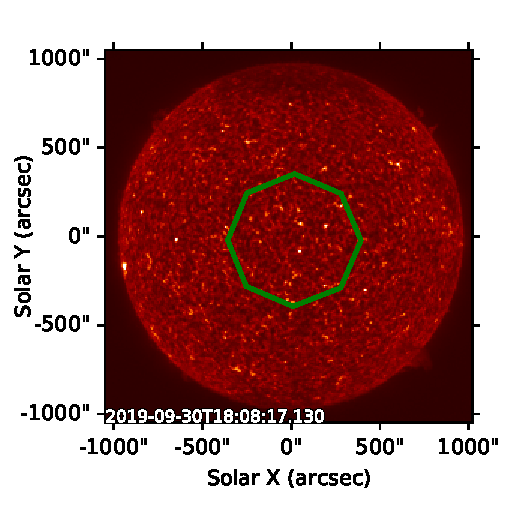
\includegraphics{esis_pointing}
				\caption{The reference AIA 304\,\AA\ data taken at 18:08:53~UT was used for determining the absolute pointing. The octagon indicates the ESIS FOV.}
				\label{fig:fov}
			\end{center}
		\end{figure}
	

		\begin{table}
		\begin{center}
			\caption{ESIS Flight Data Summary}
			\label{tab:data_info}
			\begin{tabular}{ll|ll}\hline
				Launch Date & \rts{\dateMission} & Image Size  & 2064$\times$1024 pixels \rts{\imageShape~pix}\\
				Data Acquisition Time & \rts{\timeDataStart--\timeDataStop~UTC} & Avg. Noise: & 4.0 $\pm$ 0.2 DN \rts{\readoutNoise}\\
			    Pointing   &  $\approx$ (15\arcsec, -35\arcsec) & Avg. Gain &   $2.5 \pm 0.1$\,elec DN$^{-1}$ \rts{\gain} \\
				Field of View  & $\approx 11.3$\arcmin octagonal  & Exposure Time & 10\,s \\
				Roll & $??? \pm ???^\circ$ CW & Exposure Time & 10\,s\\
			    Spatial  Plate Scale  &  \rts{\plateScale} & No. Light Exp: &\rts{\numDataFrames} \\
				Spectral  Plate Scale  &  \rts{\dispersion} & No. Dark Exp: &\rts{\numDarkFrames}\\
					\hline
			\end{tabular}
		\end{center}
		\end{table}
		
		
		\amy{Notes on this table: Change data acquisition time to full time from first dark to last dark. \rts{done.}  Change gain and noise to average +stdev of the values. \rts{done.} Correct plate scale. \rts{done.} Double check whether level1 include top/bottom 8 pixels. \rts{We do keep those 8 pixels currently. Where can I learn more about these pixels? I can't find any mention in the e2v manual.}  Double check roll and number of image.  Basically double check all values.  And why isn't it centering??}


	
\section{Data} 

    We have established several levels of data processing that are described in detail below.
    Level-0 represents the raw data that was obtained by the four different cameras during flight.
    Level-1 data prepares raw CCD data for scientific work through a quadrant dependent bias and dark subtraction and gain correction. \amy{Additionally, Level 1 will be corrected for atmospheric absorption and contain a header keyword tracking the correction as a function of time for use in instrument noise models.
    It will also be despiked, and contain a mask with the original data values for each corrected pixel for future respiking, if desired.  }

   %Level-2 data will be corrected for atmospheric absorption and contain a header keyword tracking the correction as a function of time for use in instrument noise models.
    %It will also be despiked, and contain a mask with the original data values for each corrected pixel for future respiking, if desired.
    
    \amy{Normally, for solar observatories like AIA, higher level data would be further be corrected for solar pointing and roll by interpolating the data into a standard solar map.  For ESIS this correction is complicated.  First, the effective pointing of the instrument changed from image to image due to thermal expansion of optical components during the rocket flight.  Second the data itself is complicated to represent due to the spatial-spectral overlap on the detector.  Third, to retain the most information in the data, it is desired to included detailed mapping from the solar spectral cube to each unique detector instead of shifting, rotating, or cropping the detector data.  Finally, the ESIS optical instrument distorted the solar image by design. This distortion can be measured and corrected manually, at least for the \ov data, by comparing the ESIS data to co-temporal AIA 304\,\AA\ data.  To account for  distortion for the full wavelength range requires an accurate optical model. } 
    
    Hence, we define two additional levels of data sets.  Level-2 data will include updated header information with accurate coefficients of a non-linear and wavelength dependent coordinate mapping from solar coordinates to each detector for each image.   Level-2 data is a necessary step toward inverted data products,  but will not be further described here because the results are optical model dependent and currently in development.   Instead it will be presented in a forthcoming paper.  Level-2 data will be released at the publication of that paper.  

    Instead, we seek a shortcut to interpretation of the ESIS data, which allow for taking differences between images and simplified inversions.
    Level-3 data is comprised of a single spectral line cropped from Level 1 data and mapped to the sky plane via a non-linear coordinate transform derived from comparisons with co-temporal AIA data.
    
    The highest level data product we envision providing in the future, Level-4, is the solar-spectral data cube, i.e., the intensity as a function of $[x, y , \lambda]$, which will be the results of inversions of the combined Level-2 datasets.     Since inversions generally do not produce unique solutions, there may be multiple Level-4 products obtained by different inversion methods.  Level-4 data products will be described in future publications as they become available.   
    
    Level-1 and Level-3 data will be made publicly available through various solar data archives. Below we describe these two data sets in more detail. 
    
    \amy{I am combining the Level 0 with Level 1 data description below.  I think the fact that these two are the ones that are publicly available motivates limiting the subsections to them.}
    
       
    \amy{This makes it sound like Level 3 comes from Level 1, but isn't also corrected for atmospheric absorption and despiked?  I'm going to suggest that we go back to Level 1 include atmospheric absorption correction and despiking, which I think was your plan already but I nixxed it.  SORRY !!! I have edited the text below.}
    
    %\subsection{Level 0 Data}
    %		    \jdp{This likely will need to be rearranged since some of this processing goes in to prepping the Level-1 Data.}
	     

    
    \subsection{Level-1 Data}
     %   \jdp{Don't forget to say something about tossing out the first two ESIS frames.}
	  %  \jdp{Moving Amy's comment about atmospheric absorption to this section.  Roy already has some nice plots of this and it can likely be discussed in a section explaining dark selection?}
	    
  
    
    % 	[Copied from Hi-C paper as a reminder that we need to talk about atmospheric absorption somewhere.] We use the normalized total intensities of the Level~1.0 processed flight data (processing levels described in Section~\ref{sec:data}) to assess the relative atmospheric absorption of the signal as a function of flight time.  The transmission, shown in Figure~\ref{fig:absorb} in combination with the payload altitude, is calculated as the inverse of the relative absorption (i.e., (absorption coefficient)$^{-1}$). More than 4 minutes of data were unaffected by the atmosphere.  The atmospheric absorption was compensated for in the Level~1.5 processed data set by multiplying the images by their respective absorption coefficient.  These coefficients are provided in the header of this processed set.
    	A summary of the flight data parameters, as described in the preceding sections, is provided in Table~\ref{tab:data_info}. Level-0 data is the raw data collected during the ESIS rocket flight.  
	    Each image was written to a fits files with on-board timestamp, camera number, and other parameters, such as the read out from temperature sensors included in the header.   There were (30) light images that were processed into Level 1 data and (19) dark images using to process the data.
	   
	    \amy{ We need to show an example of Level 1 data.  Two thoughts, one showing a pre and post processed data in 1 channel or an example of the post-processed data in all channels.}
	    \rts{Please see Figure \ref{fig:L0_to_L1} for an initial attempt at this figure. A challenge with this figure is that the Level-0 and Level-1 are two different sizes, so you can't share the x and y axes.}
	    
	    \begin{figure}
	    	\centering
	    	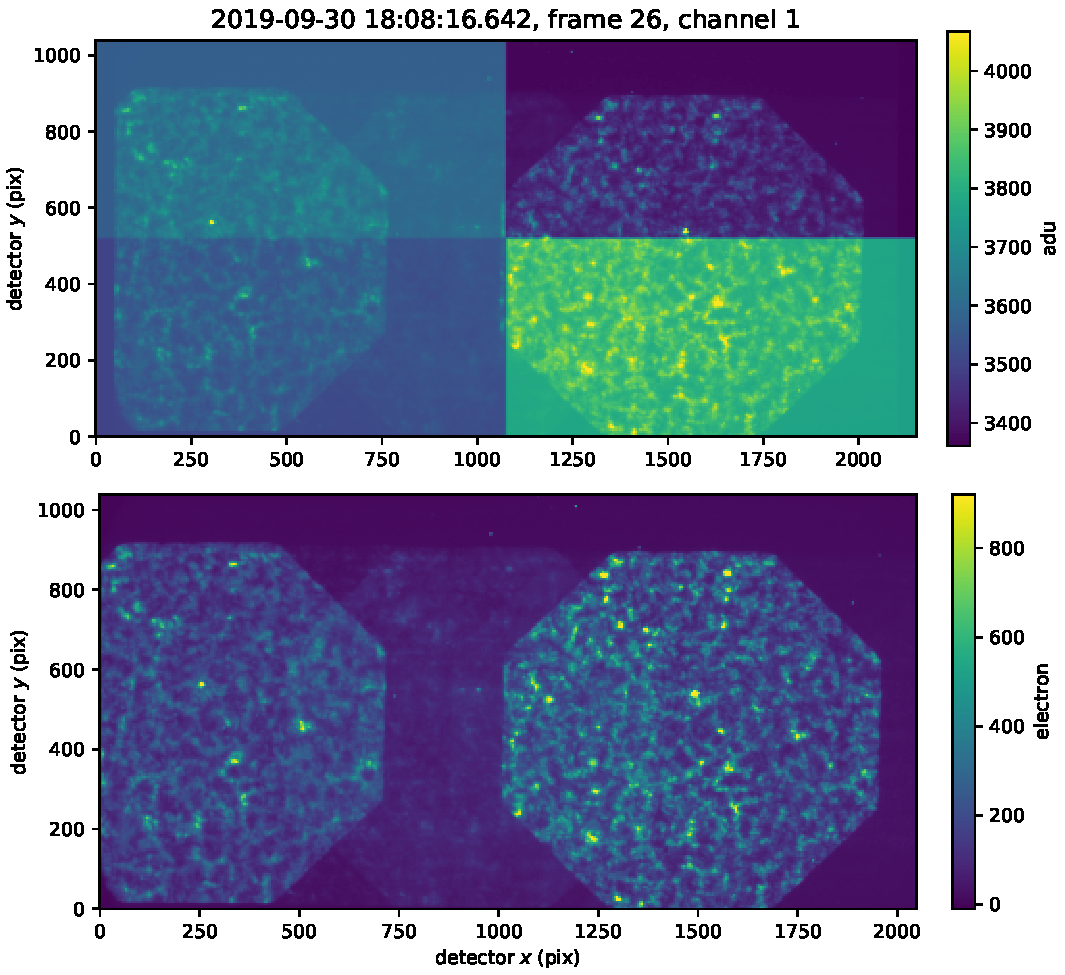
\includegraphics{L0_to_L1}
	    	\caption{The top panel is the raw, Level-0 image captured by Channel \defaultChannel\ of ESIS during apogee. The bottom panel is the same image after Level-1 processing.}
	    	\label{fig:L0_to_L1}
	    \end{figure}
    	
    	
    	The Level-1 dataset contains each channel's image sequence in units of photoelectrons.
    	Our procedure to convert from Level-0 to Level-1 is as follows:
    	
    	\begin{enumerate}
    	    \item Calculate and subtract the bias of each quadrant of each image (light or dark) by taking the median of columns 21-50 of each quadrant. Columns 1-50 are ``non-active'' pixels, and are insensitive to light or dark current. Through lab testing of the ESIS cameras, it was found that the median of columns 21-50 well-represented each quadrant's bias.  \amy{actually, don't you use the inverse on the other side of each image?} \rts{I was thinking in the coordinate system of the tap, we can change it if confusing.}
    	    \item Create a master dark image for each channel by taking the median along the time axis of all the bias-subtracted dark images taken before the shutter door opens or after the parachute deploys.
    	    \item Subtract the master dark from each bias-subtracted light image, i.e., images taken when the shutter door is open, the RLG is enabled, and SPARCS is in Fine Poining Mode.
    	    \item Crop each image to remove the non-active pixels.
    	    \item Convert images from DN to electrons by multiplying each quadrant of each image by the gain for that quadrant.
    	\end{enumerate}
    	
	In addition to the images, the Level-1 fits header is updated with the time, exposure length, and altitude associated with each image using standard FITS header keywords. \amy{but isn't that in the original level 0 fits files?} \rts{The original fits files have time at the end of the exposure, we corrected the time to the middle of the exposure. Also the exposure time was in units of ticks in the Level-0 fits file. In Level-1 the exposure time is in units of seconds.}
	
	Atmospheric absorption
	
	Despiking
	
	Maybe a list of FITS header keywords?  
	
	Units?  electrons?  will that be the distributed unit?
	
	It also strikes me that we never give a line list, though we refer to the different lines several times.  This seems like an appropriate place to give a line list?  Or in the experiment description?

    \subsection{Level 3 Data}
 
    
    	\newcommand{\vigfit}{[0.44, 0.34, 0.38, 0.5]}
    	\newcommand{\levthreetime}{2019-09-30T18:08:51.644}
    	
    	The ESIS Level-3 data product is created to provide a co-aligned, single wavelength image in each channel for quick identification of events with significant line-of-sight velocities and easy comparison with coordinated data that does not require inversion. 
    	Level-3 data also allows for single wavelength inversion prior to the completion of the final optical distortion model and the Level-2 data product.  A description of both qualitative and quantitative analysis of Level-3 data is given in Section 4.  Generating Level-3 data products require several steps including 1) correction of the optical distortion and internal co-alignment of the four ESIS channels, 2) correction of each channel for vignetting, including identifying regions where the contributions of the overlapping \mgxbright line confuse the \ov data, and 3) correcting for the relative radiometric differences in each channel.  Each of these corrections are described in detail below. 
    	Figure \ref{fig:coalign}a shows an example of a Level-3 image from Channel 1 taken at \levthreetime.
    	
  		\begin{figure}[htb!]
    		\centering
    		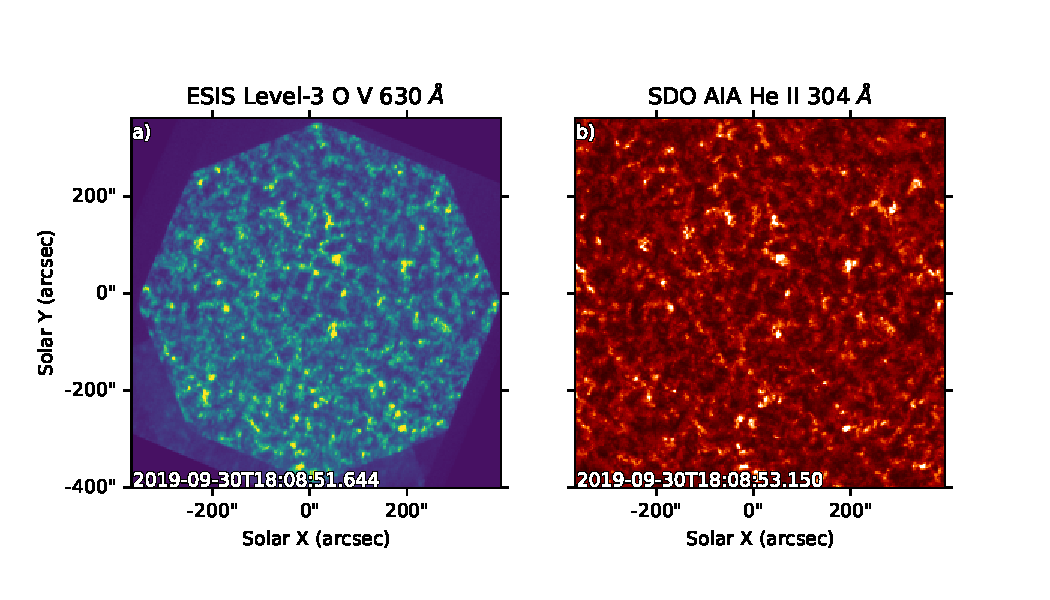
\includegraphics{aia_coalign.pdf}
    		\caption{(a) An example of the Level 3 data product from Channel 1 taken at \levthreetime. This data has been aligned using nonlinear mapping parameters to the closest co-temporal AIA 304\,\AA\ image, shown in (b).   }
    		\label{fig:coalign}
    	\end{figure}
    	
    
  \amy{We need an image of Level 1 data here, with the portion that is cropped/rotated to make 4a. It can just be part of 4 and and be above the two images or its own figure or we can include the cropped lines in hte image I suggested in the previous section.}
  
  \subsubsection{Optical distortion correction and channel co-alignmentment}
   		
   		The four ESIS channels were spatially co-aligned in two steps.  
   		First, each ESIS image is roughly cropped around the \ov spectral line and then co-aligned to the closest AIA 304\,\AA\ image in time.  AIA 304 channel was chosen for co-alignment because it is the AIA EUV channel most visually similar to O V, in both the background and bright events (Figure \ref{fig:coalign}b).
   		Prior to co-alignment each AIA image was prepped to Level-1.5 using the aiapy routines \texttt{aiapy.calibrate.update\_pointing()} and \texttt{aiapy.calibrate.register.py}  \citep{aiapy}.
   		The co-alignment was achieved through a linear coordinate transformation of the cropped ESIS image that maximizes the zero lag cross-correlation between it and AIA 304, the results of are shown in Figure \ref{fig:coalign}b.
   		Despite each image being in a different wavelength and at slightly different times we found an average zero lag cross-correlation of approximately $0.45$.
   		After the transformation each ESIS channel is re-binned to AIA resolution and can be assigned the WCS \rts{Do we have a WCS citation anywhere?}\jdp{I'll look for this.} information from AIA Level 1.5 providing pointing information and easier co-alignment with other instruments.
   		
   		%Amy- I don't think this is the right place to talk about hte contribution of Mg X.  Commenting out for now.  
   		%This rough cropping is why there is a remnant of the adjacent Mg {\sc x} 609.8 \AA \ spectral line in the bottom left corner of Figure \ref{fig:coalign}a.
   		
   		\amy{I am a little confused by this.  If after the AIA co-alignment you can assume the same WCS keywords, then you have effectively made your pixels square, your roll 0, etc.  Does the internal alignment distort this again?}
   		
    	Since ESIS has a slightly non-linear distortion function \citep{ESIS}, an additional internal alignment step is performed.
    	Using a single ESIS channel as reference, in this case Channel 2, each other channel is co-aligned to it via a quadratic coordinate transformation that maximizes the zero-lag cross-correlation. 
    	After performing this additional internal alignment we find that not only is the zero-lag cross-correlation between each channel and the reference channel improved (dots in Figure \ref{fig:cc}), but also the cross correlation between every other combination of channels (stars in Figure \ref{fig:cc}).
    	Examining the cross-correlation ratio of each camera pair shows a less than 1 percent improvement in peak correlation in Figure \ref{fig:cc}, demonstrating the subtle non-linearity of the ESIS optical distortion function.
    	In pixels, this corresponds to an average change in mapping of \jdp{\textbf{FIND THIS}}.
    	
    	\amy{This previous paragraph is confusing and needs further explanation.  Also I changed "Camera" to "Channel".  In the figure you use 0 and the first channel, is that consistent with what you are using in the text?}
    	
     	\begin{figure}[htb!]
    		\centering
    		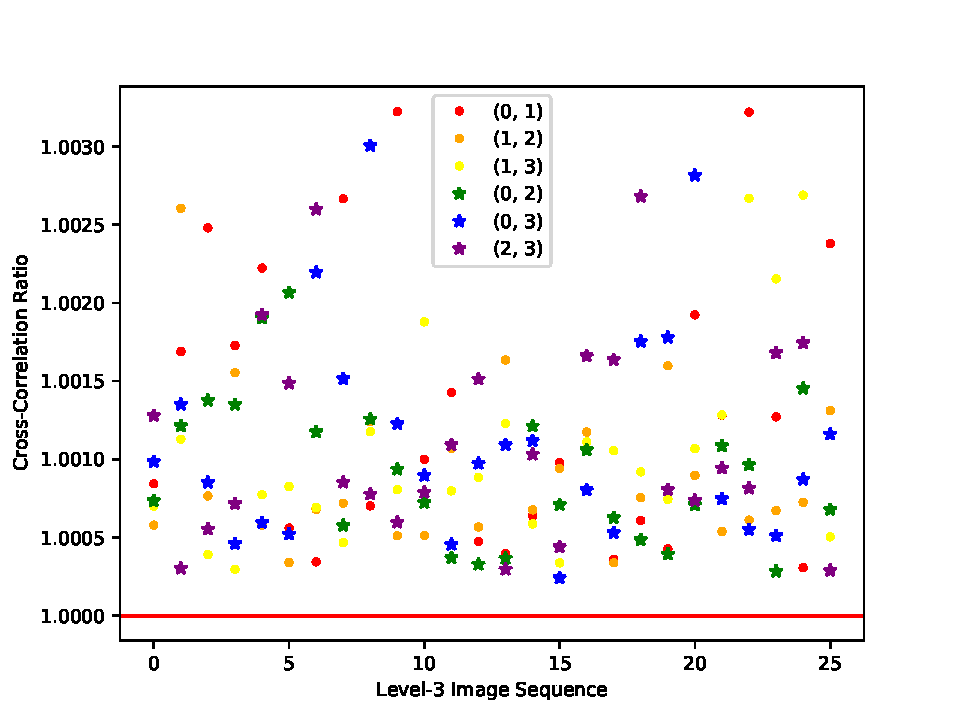
\includegraphics{internal_align.pdf}
    		\caption{For each ESIS exposure (or image sequence) every channel pair, labeled in the legend, is cross-correlated to measure internal alignment quality.  The ratio of zero lag cross-correlation after a quadratic transformation to that of a linear transformation is plotted.  Every point being above the ratio = 1 line indicates improved internal alignment for every combination of ESIS channels for each image sequence.}
    		\label{fig:cc}	
    	\end{figure}
    	
 		\begin{figure}[htb!]
			\centering
			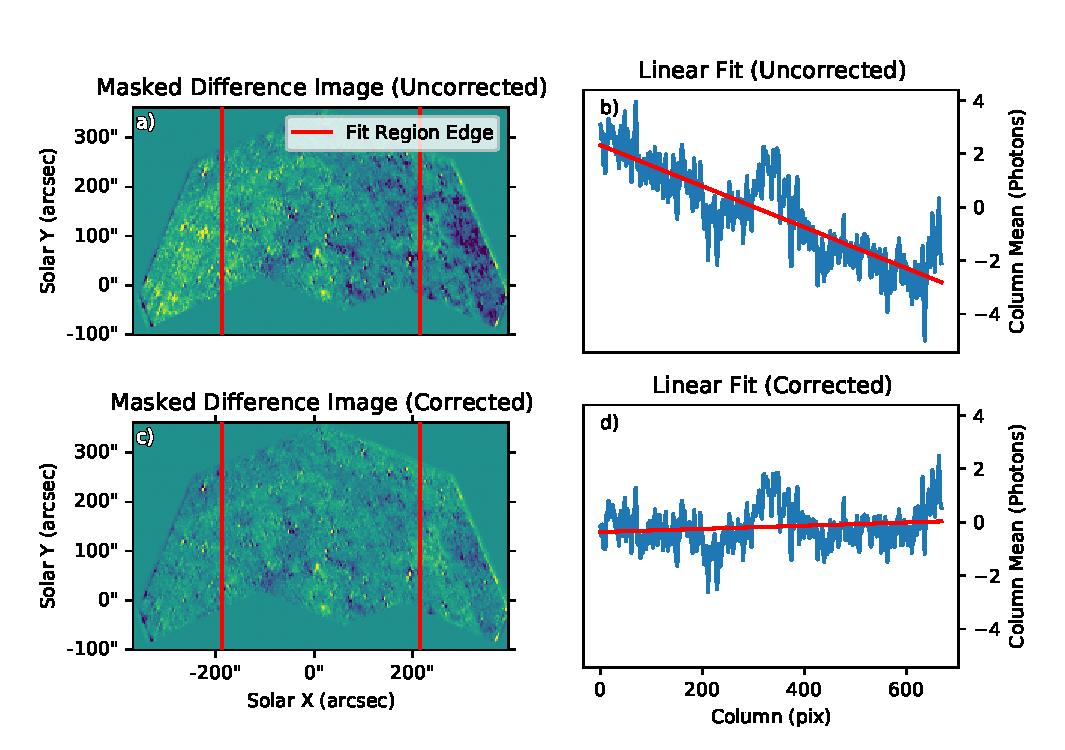
\includegraphics{vig_correct.pdf}
			\caption{Caption}
			\label{fig:vig_correct}
		\end{figure}

  \subsubsection{Vignetting correction}
  
  \amy{This section is too detailed and not detailed enough simultaneously.  You are providing a lot of information, but not enough to understand why the details you are providing are important.  Let's talk about it.  I think adding a few explanatory sentences is all that is required.}
  
        Each ESIS channel has a linear trend in intensity along the dispersion direction due to internal vignetting in the optical system due to teh central obscuration of the ESIS primary mirror and optical components \citep{ESIS}. \amy{Can you say what the vignetting is due to? I made a guess.}  In the co-aligned Level-3 where solar north is rotated to the top of the image, the dispersion axes runs at different angles relative to solar north in each channel, so the impact of the vignetting function can be seen, measured, and corrected in the Level-3 data by looking at difference images between each channel and the mean of all four channels (see the upper left of Figure \ref{fig:vig_correct}).
        \amy{What is the difference in the difference image?  Between two channels, as a function of time, between the channel mean?  Why do difference images give us information on vignetting?  I have tried to add the answer here but may not be correct.}
        
        Measuring the vignetting function from the data is additionally complicated by the overlap of the bright \mgxbright line.  This line overlaps different regions of the field of view in each channel, see Figure~\ref{fig:mgx_overlap}.  To  better estimate the vignetting, then, we restrict ourselves to the portion of the field of view without the \mgxbright overlap in any channel.  
        
        %To correct the trend, we divide out a linear trending background from each image with a slope oriented to the dispersion direction in each channel.
        %The vignetting field divided out for each channel is,
        We define the vignetting field for each channel, $i$ at each time, $s$, as a function of the pixels in the Level-3 data, $(x,y)$, as 
        \begin{equation}
            V_{is}(x,y) = m_{i} * [r(x,y,s) - r_0] + 1,
            \label{eqn:vignet}
        \end{equation}
       	where
       	\begin{equation}
       		r = x_0 + [\cos(\alpha_i)(x-x_0-x_{\text{drift}}*s) - \sin(\alpha_i)(y-y_0-y_{\text{drift}}*s/s_t)].
        	\label{eqn:vignet2}
       	\end{equation}
       	
       	In Equation \ref{eqn:vignet}, $r_0$ is equal to 65 pixels, and represents the distance from the Level-3 image edge to the ESIS field stop octagon edge at $s = 0$, the first Level-3 image sequence.
       	The slope of the vignetting field for each channel, $m_{i}$, is a free parameter of the fit.
        In Equation \ref{eqn:vignet2},  $\alpha_i$ is the angle of rotation of each ESIS Level-3 image relative to a Level-1 image row.
        In this case, $\alpha_i = [112.5^{\circ}, 67.5^{\circ}, 22.5^{\circ}, -22.5^{\circ}]$ for Channels 1-4, respectively.
        The vignetting field is rotated about the origin of each image in pixels, $[x_0, y_0] = [635,635]$, to account for the change in dispersion direction.
        Because ESIS images have a slight pointing drift, causing the octagon to move as a function of time, as a function of time, or image sequence $s$, the image origin is translated by $[x_{drift},y_{drift}]*s/s_t = [8_{pix},-4_{pix}]*s/29$, where $s_t $ is the total number, \numDataFrames, of Level-3 images in time. \amy{I think there might be a simpler way to give this last equation on teh drift.  And why does the vignetting depend on solar pointing?}
        
        \begin{figure}[htb!]
        	\centering
        	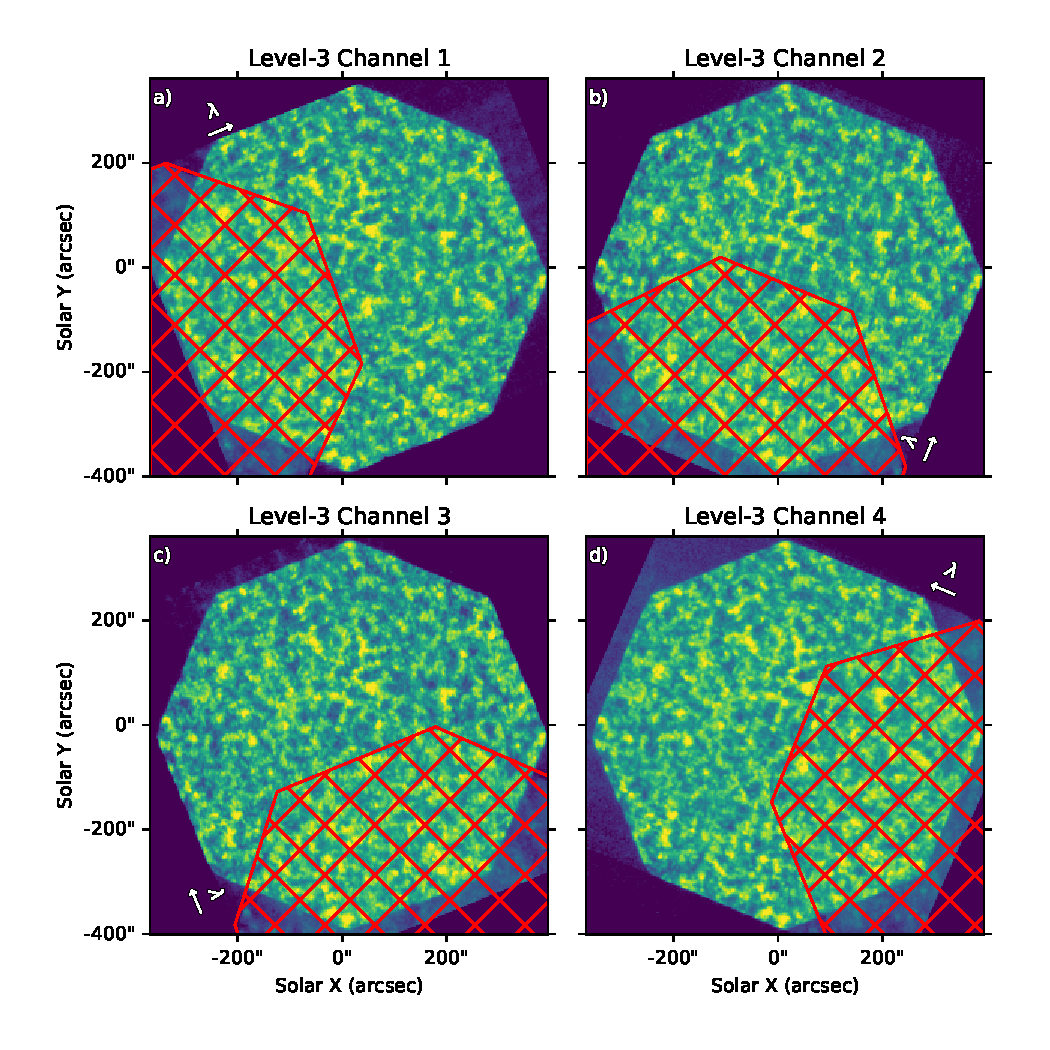
\includegraphics{mgx_overlap.pdf}
        	\caption{The red hashed region shows the overlap of the Mg {\sc x} 609.8 \AA \ spectral line in each channel that is masked prior to the vignetting correction and intensity normalization. These images are displayed in log scale in and attempt to bring out the subtle contamination.  The outline of the Mg {\sc x} can be seen very clearly in difference images like Figure \ref{fig:l3_dif}. }

        	\label{fig:mgx_overlap}
        \end{figure}
        
        When fitting for the vignetting field slope, $m_i$, for each  of the four ESIS channels we mask off the portion common to them all with no contribution from \mgxbright.
        The four channels of ESIS give 6 possible difference images for fitting the vignetting function for each image sequence $s$. 
        For each difference image we take a mean of each column and fit a line to it as a function of column position, shown in the right hand column of Figure \ref{fig:vig_correct}.
        When the average slope of all 156 fits (6 difference images per each of the 26 exposures) \amy{here you say 26 exposures, above you say 29.}
        is minimized we consider the vignetting corrected. 
        The resulting final fit, $m_i = \vigfit$, gives smaller slopes than are predicted using ray tracing and geometric optical models \citep{ESIS}, which can be attributed to a few likely culprits. \amy{in Figure 6 b, you give a slope of -2.54, why is it so different from these numbers?}
        One source of error likely comes from the imprint of adjacent spectral lines, the most obvious being that of Mg {\sc x} 626 \AA \ visible in Figure \ref{fig:vig_correct}c.
        Since this Mg {\sc x} line overlaps almost entirely with O {\sc v}, and has an identical vignetting function, it adds intensity that prevents a perfect fit. 
        If this were the only source of discrepancy between the vignetting function predicted by the raytrace and the fits obtained from the data, then we would simply use the same, predicted vignetting for every channel. 
        However, we can anticipate slightly different vignetting in each channel due to variations in assembly so we allow each channels slope to vary independently.
        A misalignment of the ESIS field stop center, the ESIS primary optic center, and the center of the ESIS grating array, all shift the geometry of the ESIS central obscuration and can easily modify the vignetting field in each channel.
        Despite the uncertainties in vignetting, which we have found difficult to quantify, Level-3 differences are much flatter in intensity post vignetting correction as is seen in Figure \ref{fig:vig_correct}c, and will therefore lead to a higher fidelity intensity recovery when inverting Level-3 data.
        
       	\subsubsection{Relative Radiometric correction }	 
   		In order to use Level-3 data for early inversion the intensity in DN needs to  converted to photons in order properly account for uncertainty and then normalized between channels.
   		Since each ESIS CCD has a quadrant specific gain \citep{ESIS}, the conversion from DN to photon is done to Level 1 data prior to co-alignment efforts.
   		The intensity in photons for each quadrant, $I_q$, then becomes,
   		\begin{equation}
	   		I_q = I_{DN} * G_q * 3.6\ \frac{\SI{}{\electronvolt}}{\SI{}{\elementarycharge}} * \frac{\lambda}{hc}.
   		\end{equation}
		With an average quadrant gain, $G_q$, of \SI[per-mode=symbol]{2.56}{\elementarycharge\per\electronvolt}, a Silicon band gap energy of \SI[per-mode=symbol]{3.6}{\electronvolt\per\elementarycharge}, and an energy per \ov photon of \SI[per-mode=symbol]{19.6}{\electronvolt\per\photon} gives each count in $DN \approxeq 0.46$ photons.
		Creating Level-3 data for other wavelengths in the ESIS passband then only requires a different wavelength for conversion.
   		Normalizing the intensity of each channel is done by equalizing the image mean over a shared piece of sun, and is therefore performed after inter-channel co-alignment. \amy{And vignetting correction?  If the conversion from DN to photon is done in Level 1, why isn't it discussed there?  For Level 3, only the last sentence is needed, no?  I think you want to point out the you only use the region where MG X bright is not.}
  

\section{Preliminary Results}

	   ESIS is an extremely unique instrument.  It is not only a slitless imaging spectrograph, of which there only a handful of examples, it is also a Computed Tomographic Imaging Spectrograph (CTIS).  The ESIS and MOSES sounding rocket instruments are the only CTIS instruments ever to observe the Sun. MOSES only took two projections of the spatial-spectral data cube by observing $\pm$ 1 orders, so its data is relatively simple when compared to the ESIS data set.   In this section, we provide some preliminary analysis of the ESIS Level-3 data to both demonstrate that the ESIS mission accomplished its scientific goal of detecting the velocity signatures of small scale eruptive events, but also to provide useful qualitative and quantitative understanding of this data.  
		
	    Despite the lack of solar activity, ESIS managed to capture tens of small, transient events and one significant eruption during the $\approx$5 minutes of observation in the \ov spectral line.  We provide a few examples of these events in this section.  Additional analysis is provided in a series of upcoming papers.  
	
    \subsection{Level-3 Difference Images}
    	Early work with MOSES images demonstrated the utility of examining difference images between different projects of the spatial-spectral cube (channels) to identify solar features with significant line-of-sight velocity \citep{Fox2010,FoxPhD,RustPhD,Rust2019}, and extra spectral content \citep{RustPhD, Rust2019,Parker2021}.  \amy{what does extra spectral content mean?}
    	It is for this reason that we developed a spatially co-aligned data product (the Level-3 data) quickly that would allow us to take differences between each ESIS channels.
    	Each ESIS channel disperses solar features in a different direction relative to solar north, determined by the azimuthal position of each grating.
    	The positive dispersion direction in each Level-3 image is indicated by the arrows  in Figure \ref{fig:mgx_overlap}.
    	In the case of an eruptive event with a velocity signature, the Doppler shift is dispersed a different direction in each channel, meaning taking the difference between two spatially aligned channels leave only intensity away from the spectral line core.  To put it another way, subtracting the data from two channels removes all the spatial structures that overlap in the two channels and leaves only the velocity signatures.  \amy{I don't know if this is helping, but feel this needs additional description.}
    	%For our initial analysis, we focus on the dominant O {\sc v} 629.7 \AA \ spectral line in the ESIS passband. \amy{I think this is a given since it is the only one in level3}
    	
    	Figure~\ref{fig:l3_dif} shows the difference between Channels 2 and 3 for the full ESIS field of view.  Several regions of the field of view show black and white features, a few of these are marked with red boxes and will be discussed in detail below.  The small black features tend to lie at an angle -22.5$^\circ$ with solar north, which is the direction of dispersion of Channel 3, while white features tend to lie at an angle of 22.5 $^\circ$ with solar north, which is the direction of dispersion of Channel 2.  Due to the relative orientation of each ESIS channel's dispersion axis, taking the difference of these small events leaves a V-shaped or X-shaped structure in it's place.  Every X or V-shaped features in an ESIS difference image, Figure~\ref{fig:l3_dif}, that have obvious, and nearby, positive and negative portions indicate solar events with significant line-of-sight (LOS) Doppler velocity.   Other things to note in this image is the white octagon that overlays the lower left quadrant of the image, this is the \mgxbright line that overlaps the \ov line in Channel 2.  The dark octagon on the lower right quadrant is the portion of the \mgxbright line that overlaps the \ov line in Channel 3.    
   		
   		\begin{figure*}[htb!]
   			\centering
   			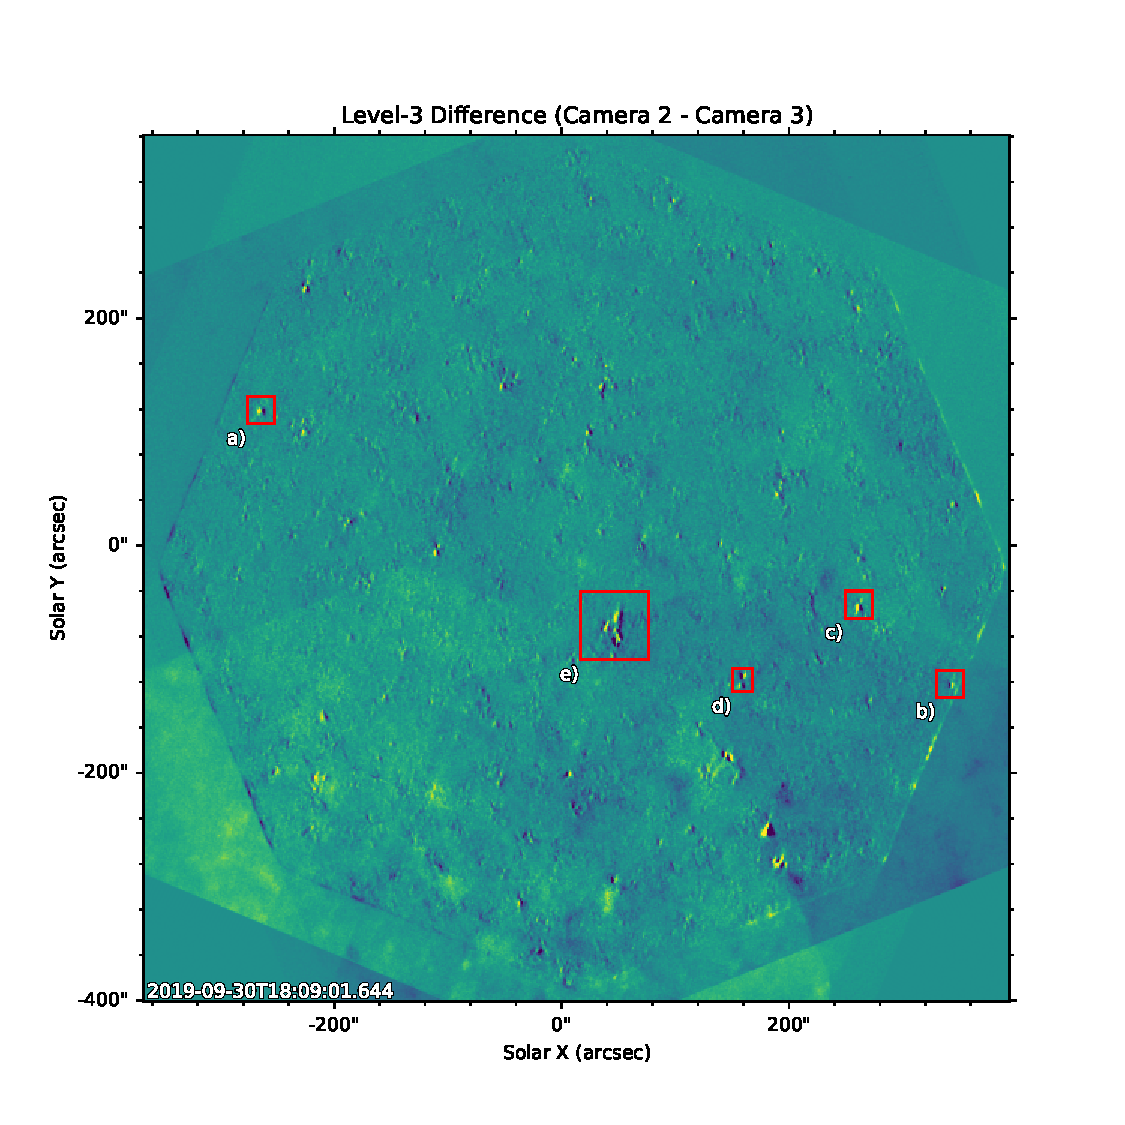
\includegraphics{l3_dif}
   			\caption{Full FOV Difference between Channel 2 and Channel 3 Level-3 images.  Events a-c are highlighted in Figure \ref{fig:dif_events}.  A time series of Event d is shown in Figure~\ref{fig:main_event}.}
   			\label{fig:l3_dif}
   		\end{figure*}
   	
 		\begin{figure}[htb!]
   			\centering
   			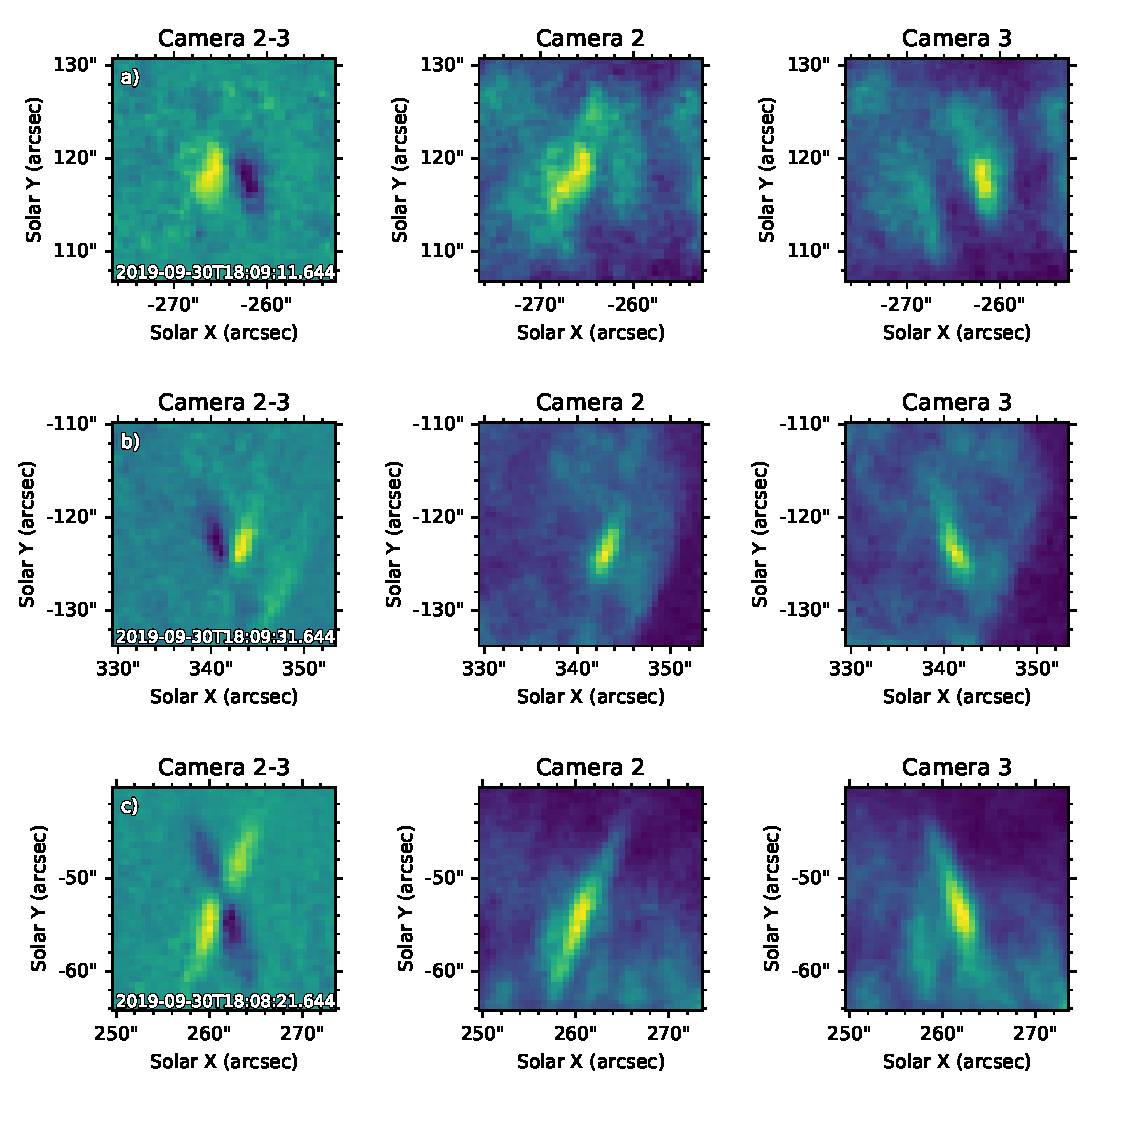
\includegraphics{dif_events}
   			\caption{Events a, b and c identified in Figure \ref{fig:l3_dif} are examples of a mostly blue, red, and broadened even, respectively. The difference between Channels 2 and 3 is shown in the left hand column, while the Channel 2 and Channel 3 intensities are shown in the middle and right columns.  The velocity signature is most easily seen in the difference image, while the straight intensities provide information on the line core intensities. 
   			    \rts{You should share y-axes to save space here I think.} \amy{You use camera instead of channel everywhere.}
   			}
   			\label{fig:dif_events}. 
   		\end{figure}

    	Simple, point-like, transient brightenings with little or no spatial structure are the easiest events to interpret because their naturally confined spatial extent acts similarly to a spectrographic slit.
    	Therefore, any spatial extent in an ESIS image is mostly due to spectral dispersion. \amy{I think the previous sentence is confusing.}
    	In these simple events, a qualitative understanding of their velocity can be ``read off'' of each ESIS image.
    	This is effect was explored in great detail by \citet{Rust2019}, who sliced through these small events along the dispersion direction and measured line profiles.
    	
    	Here we explore the velocity signature in three examples of simple point-line events marked a-c in Figure~\ref{fig:l3_dif}.  Figure \ref{fig:dif_events} shows the difference image in the first column for all three events, then the Channels 2 and 3 data in the subsequent columns. Figure \ref{fig:dif_events}a shows a V-shaped event that is pointed downward in the difference between the Channel 2 and Channel 3 Level-3 image.
    	Since we know that the direction of positive wavelength dispersion is up and to the right in Channel 2 and up and to the left in Channel 3 (Figure \ref{fig:mgx_overlap}) we immediately know that this event is predominantly blue shifted.  
    	Similarly, an upward facing V-shaped event, like the one shown in Figure \ref{fig:dif_events}b, is predominantly red shifted.
    	X-shaped events, shown in Figure \ref{fig:dif_events}c, that occur equally if not more frequently than V-shaped events, indicate significant line broadening. \amy{suggest enhanced emission in both the red and blue wing of the line profile?}
    	Difference images can provide immediate qualitative understanding of these simple, point-like events.  During the 5 minute rocket flight, tens of similar events were detected in the ESIS field of view.  
    	
    	%While this gives us a quick and qualitative understanding of a simple event, even the smallest amount of spatial extent in a given feature leads to an entanglement of spatial and spectral information making it very difficult to derive qualitative velocities without inversion. 
    	
    	\begin{figure}[htb!]
    		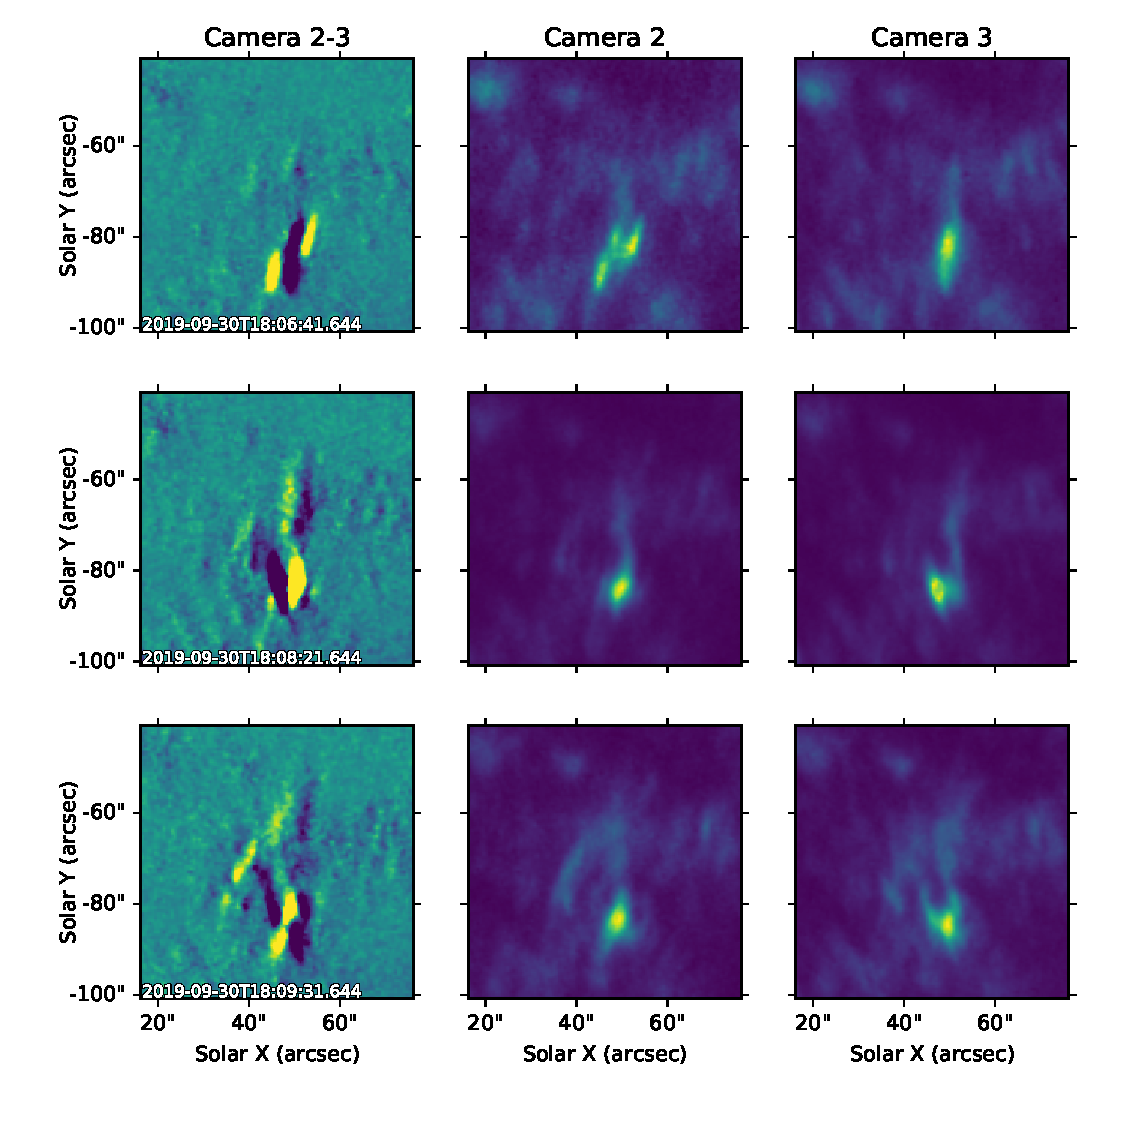
\includegraphics{main_event}
    		\centering
    		\caption{The largest eruption captured by ESIS shown at three different times. The event starts with a bidirectional flow with slight spatial separation, evolves into a strong red shift }
    		\label{fig:main_event}
    	\end{figure}
		
    	During the ESIS flight, we also captured a handful spatially extended objects that are more difficult to interpret.
    	The most obvious of these is an eruption near disk center, event d in Figure \ref{fig:l3_dif}.
    	This large event is shown at three times in Figure \ref{fig:main_event}.
    	As shown, an erupting two-dimensional feature leads to an entanglement of spatial and spectral information that makes it very difficult to derive qualitative velocities without inversion.
    	In difference images (left column) there is a mess of positive and negative features intertwined in the brightest portion of the event that sometimes present as a V or X shape, but not always, and evolve significantly in time.
    	The top row shows this event early in it's evolution. 
    	Intensity is concentrated to a small region and presents as two jets, one red and one blue, with a slight spatial separation.
    	Shortly after (middle row) the event is dominated by a significant red shift (upward facing V) at the location of initial brightening, 
    	There is also an imprint of fainter differences above the brightest knot of intensity showing motion along a spatially extended structure.
    	The difference in this faint structure is opposite in polarity to the intensity below, and therefore appears to be ejected blue shifted material from the site of initial brightening.
    	By the end of the event (bottom row), the dominate red shift subsides, leaving a complicated spectral signature and the brightest portion of the event, and in adjacent region up and to the left.  
    	Dynamic and spatially extended events are excellent opportunities for ESIS to shine and clearly demonstrate the need for many different projection angles (ESIS channels) if we hope to disentangle spatial information from spectra.
    	Despite the extra complexity, an understanding of ESIS difference images provides an excellent sanity check when interpreting future inversions.
    	
    
    	Larger positive or negative features with no obvious counterpart nearby, are indicative of extra spectral content \citep{RustPhD,Parker2021}.
    	The most easily seen impact of this is a faint octagon edge visible in Figure \ref{fig:l3_dif} from Mg {\sc x} 625.9 \AA.
    	Extra spectral content will act as a source of error when inverting Level-3 data, but will be properly accounted for by a wavelength dependent optical distortion model and the completion of the ESIS Level-2 data set \citep{Smart2022}. 	 
    	\amy{roy's paper already slated for 2022?  I mention some of this above, don't know if we need to keep it in both places.}
    
    
    \subsection{Early Inversions}
    	In order to better disentangle the spectral and spatial information captured by ESIS, information from every channel is combined and ``inverted'' to return a single, spatial-spectral cube, at every exposure.
    	For out preliminary inversions of ESIS Level-3 data we used a Multiplicative Algebraic Reconstruction Technique (MART).
    	MART is attractive for our first inversions because it is fast, requires no training or assumptions about the data, and automatically enforces image  positivity.
    	We describe our particular implementation in more detail in Appendix \ref{MART}.
    	
    	\begin{figure}[htb!]
    		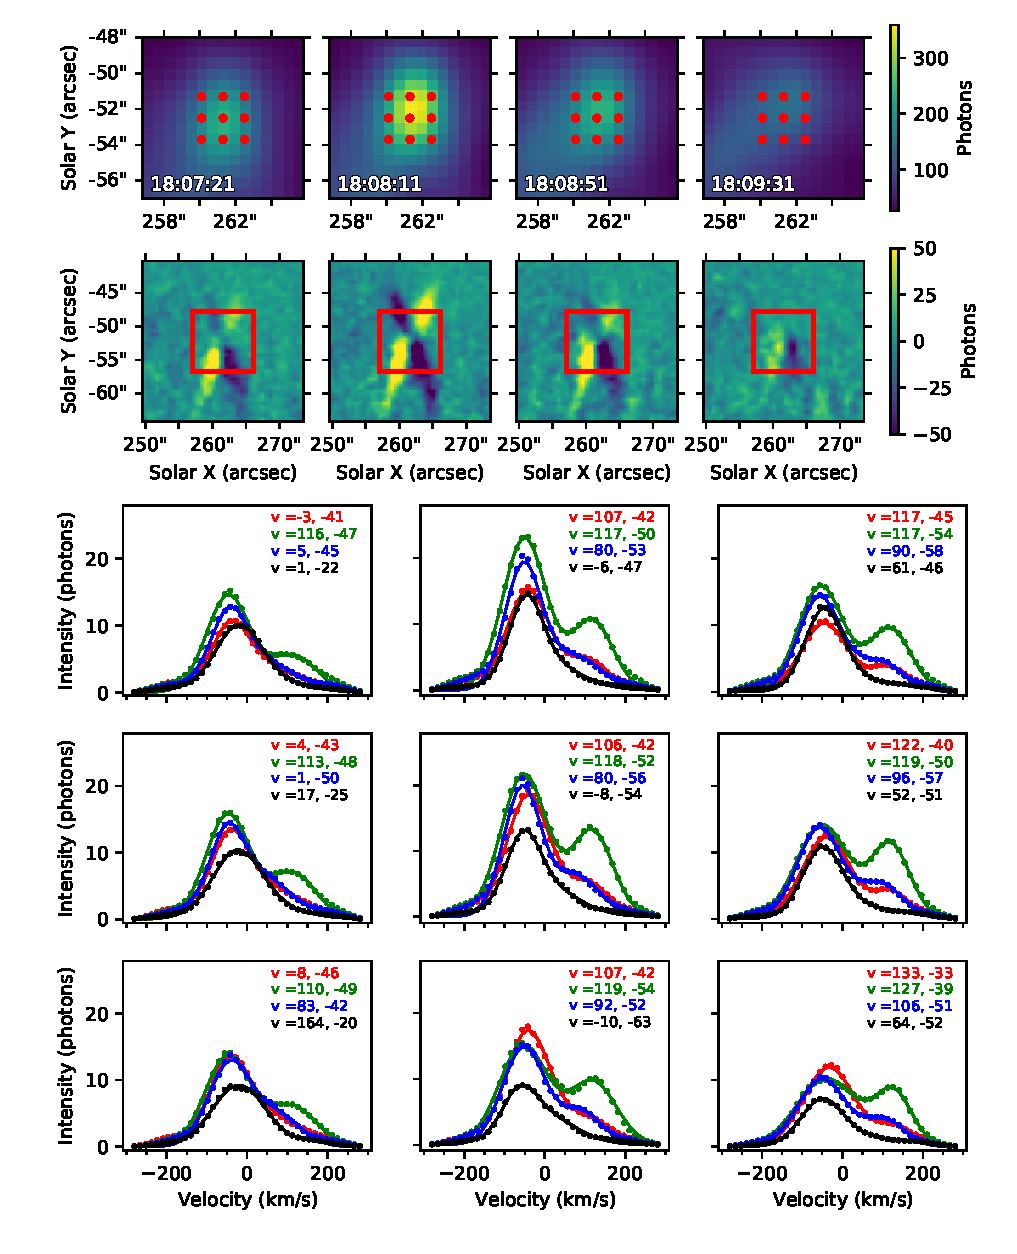
\includegraphics{perfect_x_inverted}
    		\centering
    		\caption{MART inverted results of event c in Figure \ref{fig:l3_dif}. The integrated intensity (top row) and corresponding Level-3 difference image (second row) are shown at 4 different times. A red box on each difference image marks the FOV used in the top row.  The \ov line profile at each position marked with a red dot is plotted in the matching 3x3 grid in a different color for each time (in order red, green, blue, black). Each MART line profile (dots) is overplotted with a double gaussian fit (solid line).  Bulk shifts in km/s for each component of the fit are added for each time in their respective color. }
    		\label{fig:perfect_x_inverted}
    	\end{figure}
        
        \begin{figure}[htb!]
    	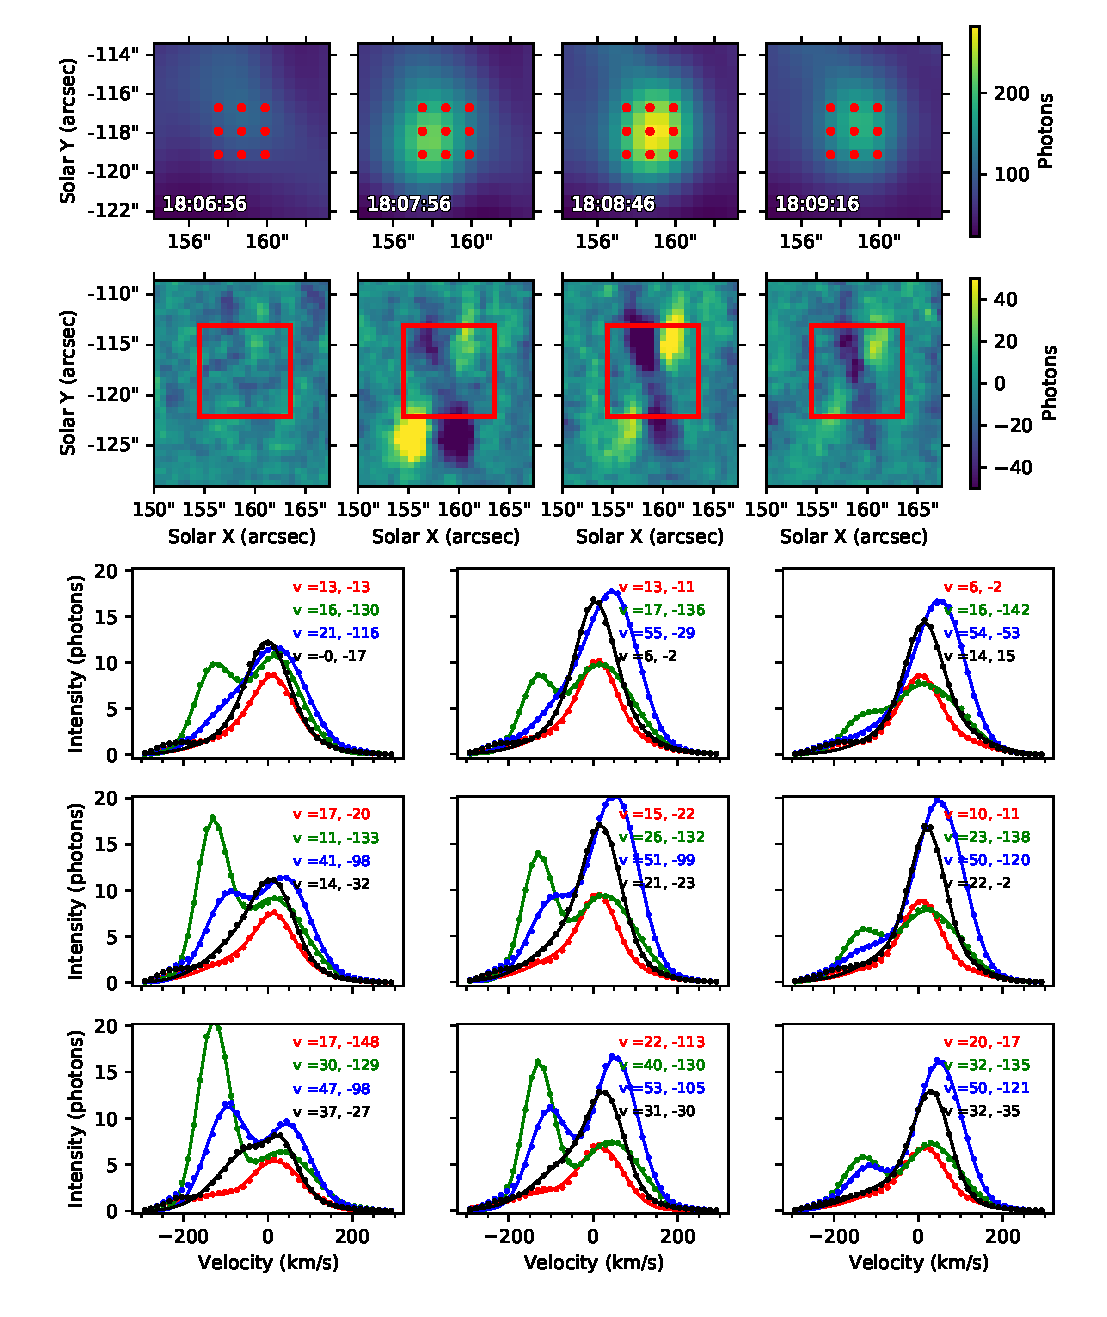
\includegraphics{other_x_inverted}
    	\centering
    	\caption{MART inverted results for event d in Figure \ref{fig:l3_dif} presented in the same fashion as Figure \ref{fig:perfect_x_inverted}.}
    	\label{fig:other_x_inverted}
    	\end{figure}
    	
    	In Figures \ref{fig:perfect_x_inverted} and \ref{fig:other_x_inverted}, and their associated animations, we present the MART inversion for two different compact transient events, labeled c and d in Figure \ref{fig:l3_dif}.
    	Both events have an X-shaped presentation, begin and end within the ESIS observing time, and show noticeable temporal evolution in velocity.
		Each figure shows the total integrated intensity (top row) and Channel 2-3 Level-3 difference image (second row) at four different times.  
		The FOV of the integrated intensity is shown as a red box on the difference image below. 
		Inverted \ov line profiles at each spatial location marked by a red dot in the integrated intensity image are plotted in the matching 3x3 grid for each time (in the order red, green, blue, black).
		We performed a double gaussian fit for each line profile (solid line) and plotted it over the MART inverted data (dots).
		The deviation from line center of each gaussian is recorded in km s$^{-1}$ in the color matching line profile.
		In the animation, we plot the red and blue components of each fit separately as dashed lines, their sum as a solid line in fuschia, and the MART inverted line profile in  
		
		Event c described Figure \ref{fig:perfect_x_inverted} lasts just over 4 minutes and shows significant temporal evolution in the line profile.
		Throughout the event the blue component of the \ov line dominates and is centered at $\approx$ -50 km s$^{-1}$.
		This blue component persists for the entire duration of the event with very slight deviations intensity and velocity.
		The red component of the event is bursty in nature, with two small peaks in intensity at 18:07:41 and 18:08:11, and is centered at $\approx$ 110 km s$^{-1}$.
		While there are a several frames where the red component of the line appears as an additional peak in the line profile and is well fit by a second gaussian, most of the time it presents more as an asymmetric broadening in the red wing of the line making the velocities from the fit less reliable.
		This explosive event covers is $\approx$ 3 arcseconds in diameter and show little spatial variation in the line profile across the event.
		
		The explosive event highlighted Figure \ref{fig:other_x_inverted}, event d, is similar to event c in that is has enhancements in both the red and blue wing of the line profile, but is more complicated in it's presentation.
		Event d  begins at 18:07:11 and it's intensity has almost completely died away by the last Level-3 image, but not entirely. 
		\jdp{verify after Level-3 rebuild}
		A strong blue component in the line profile centered near -125 km s$^{-1}$  peaks at 18:08:01 dominates early in the event evolution.
		This blue component is brightest in the lower left portion of the event.
		The red component of the line profile peaks at 18:08:51 and is centered near 50 km s$^{-1}$.
		Unlike event c, the blue component of the line is less persistent in time.
		Also, the blue and red components of the event do not occur in the same spatial location.
		This is visible both in the grid of line profiles and the difference images.
		Intensity in the line profiles show the blue component peaking in the lower left, while the red component peaks in the middle to right columns.
		In the difference images there is a clear vertical and horizontal separation between the blue downward facing V and the red upward facing V. 
		A closer look at the inverted data shows an $\approx$ 1.35 arcsecond spatial separation between centroids of the blue and red component.  
    	
    	
    			
    		   	
    	
\section{Discussion/Conclusions and Future Work}





\appendix
\section{Multiplicative Algebraic Reconstruction Technique}\label{MART}
	\jdp{Now that this is floating more, I'll need to add a few things about MART and why it is attractive for this type of problem.}
	MART adds an additional smoothing step to a simple MART applied in the past to limited-angle tomography problems like ours \citep{Okamoto1991,Verhoeven1993}.
	When testing a variety of inversion methods on MOSES data \citet{FoxPhD} identified MART as most promising of several methods in terms of speed and fidelity.
	\citet{RustPhD} applied a slightly different version of MART to the MOSES data paired with a wavelet based partial reconstruction technique for better background subtraction and event isolation.
	
	With MART we seek to reconstruct the true spatial-spectral cube, $I_{xy\lambda}$, using every ESIS image or projection, $f_{\theta x'y'}$. There is one ESIS image for each $\theta$ representing the relative orientations of each ESIS channel. The procedure is executed as follows:
	\begin{enumerate}
		\item \label{step:guess} Create a guess cube, $G_{xy\lambda} = 1$ on the same domain as $I$. 
		\item \label{step:contrast} Enhance the contrast of $G$ and normalize. 
			\begin{equation}
				G \leftarrow \frac{G+G^{(1+\Psi)}}{\sum_{xy\lambda}G+G^{(1+\Psi)}}\sum_{xy\lambda}G, 
			\end{equation}
		
		\item \label{step:smooth} Convolve $G$ with smoothing kernel $K$, $G \leftarrow G * K$,
		in our case,
			\begin{equation}
			\label{eq:kernel}
				K_{ijk} = \frac{2^{3-|i|-|j|-|k|}}{64} \quad \text{for}\quad i,j,k = -1,0,1.
			\end{equation}
		
		\item \label{step:project} Sum $G_{\theta xy\lambda}$ along lines of constant $x-\delta\lambda$ to calculate a projection for each angle $\theta$,
			\begin{equation}
				f'_{\theta x'y'} = \sum_\lambda G_{\theta(x-\delta\lambda)y\lambda}, 
			\end{equation}
		where,
			\begin{equation}
				G_{\theta xy\lambda} = \mathcal{R}_\lambda(\theta)\,G_{xy\lambda},
			\end{equation} 
		and, $\mathcal{R}(\theta)$, is a rotation about the $\lambda$ axis. 	
		
		\item \label{step:chisquared} Calculate reduced chi-squared for each projection and check for convergence, in this case that $\chi_{R,\theta}^2 < 1$ , 
			\begin{equation}
				\chi_{R,\theta}^2 = \frac{1}{N_{x'} N_{y'}}\sum_{x'y'} \frac{(f_{\theta x'y'}-f'_{\theta x'y'})^2}{f'_{\theta x'y'}+\sigma^2_{RN}},
			\end{equation}
		where $\sigma^2_{RN}$ is the read noise in photons squared, $N_{x'}$ is the total number of elements along $x'$.
		
		\item Calculate correction factors for each unconverged channel, $\theta_{uc}$, weighted by $\gamma$, 
			\begin{equation} \label{eq:correctionfactor}
				c_{\theta x'y'} = \left[\frac{f'_{\theta x'y'}}{f_{\theta x'y'}}\right]^\gamma,
			\end{equation}
		where $\gamma = 2/n$ with $n$ equal to the total number of channels.
		
		\item Assign correction factors to lines of constant $x-\delta\lambda$ in the domain of $G$,
			\begin{equation}
				C_{\theta (x-\delta\lambda)y\lambda} = c_{\theta x'y'}
			\end{equation}	
		
		\item \label{step:correct} Apply a weighted product to each derotated correction to $G$ ,
			\begin{equation}\label{eq:correct}
				G \leftarrow G\left\lbrace  \,\prod_{\theta=\theta_{uc}}  \mathcal{R}_\lambda(-\theta_i)C_{\theta xy\lambda} \right\rbrace^{1/m_{uc}},
			\end{equation}
		where $m_{uc}$ is the total number of unconverged channels and 
		
		\item Repeat steps \ref{MART}\ref{step:contrast}-\ref{MART}\ref{step:correct}
		until every channel has converged at step \ref{MART}\ref{step:chisquared}.
	\end{enumerate}
		For this particular implementation we use a contrast enhancement exponent of $\Psi = .2$ and have a total number of channels, $n=4$.
		The spectral dispersion of an ESIS grating, $\delta$ is equal to 28 m\AA\ pix$^{-1}$. 
		We construct $G$ such that its resolution \jdp{bin size? step size?} in $\lambda$ is equal to $\delta$.
		All negative values introduced by rotation are set to zero after each rotation.

